$subject$=Физические основы компьютерных \\ и сетевых технологий
$teacher$=Лекции Зинчика А. А.
$date$=08.09.2025

Всего существуют 3 способа поляризации:

\begin{enumerate}
    \item Поглощение (или дихроизм): свет проходит через вещество с длинными нитевидными молекулами. Проходя вдоль молекулы, свет свободно проходит, а поперек молекул свет не проходит

    Большинство таких линейных поляризаторов (или так называемых поляроидов) состоят из полимерной пленки или частиц кристаллов турмалина или герапатита в нитроцеллюлозной пленке

    \item Преломление: в призме Николя используется двойное лучепреломления света. В ней используется анизотропный кристалл исландского шпата, в котором

    \begin{itemize}
        \item лучи, поляризованные горизонтально, имеют показатель преломления $n_o = 1.66$ -- их называют обыкновенными
        \item лучи, поляризованные вертикально, имеют показатель преломления $n_o = 1.51$ -- их называют необыкновенными
    \end{itemize}

    Призма Николя представляет собой две одинаковые треугольные в сечении призмы. Обыкновенный луч испытывает полное внутреннее отражение от склеивающего слоя с $n = 1.55$ и поглощается, а необыкновенный свободно проходит через него и вторую призму, так как показатели преломления приблизительно равны

    % TODO картинка

    \item Отражение: Столетов предложил сделать поляризатор из стекла. При определенном угле падения $\alpha = \arctg n$ (известном как угол Брюстера) отраженный свет получается поляризованным. Для стекла этот угол равен примерно $59^{\circ}$, однако отраженный свет получается с интенсивностью 4\% от интенсивности входящего света.

    Столетов предложил использовать несколько стеклянных пластин, чтобы увеличить интенсивность -- данное устройство, состоящее из стопки стекла, получило название стопа Столетова

    Угол Брюстера применяется в изготовлении лазеров для получения поляризованных волн 

    % TODO картинка
\end{enumerate}

\section{Лекция 2. Дисперсия света}

Дисперсией света называется зависимость показателя преломления от частоты волны света

Данных эффект был обнаружен Исааком Ньютоном при разложении света в спектр. Тогда Ньютон обнаружил, что для разных частот света (а следовательно для разных волн) показатель преломления разный, поэтому в стекле лучи разных частот двигаются с разной скоростью, на выходе призмы получается радужный спектр 

Благодаря дисперсии существует радуга: лучи Солнца, проходя под определенным углом (42 градуса над горизонтом) через капельки воды в воздухе, раскладываются в спектр и попадают на сетчатку глаза

\begin{wrapfigure}{R}{0pt}
    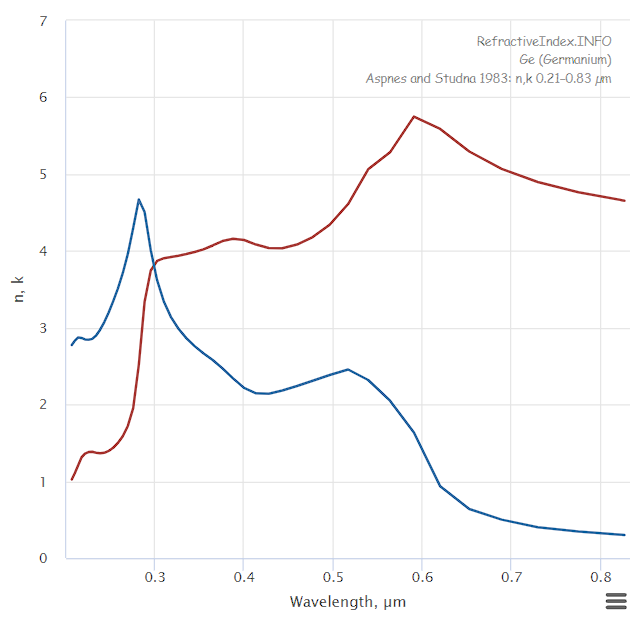
\includegraphics[width=6cm]{physics3/images/physics3_germanium_refractive_index}
\end{wrapfigure}

На сайте \url{https://refractiveindex.info} можно узнать показатель преломления. Например, металл германий, использующийся в тепловизорах, имеет показатель преломления 3.5-4 в инфракрасном спектре волн, что улучшает разрешение тепловизора при ограниченном объёме устройства

Подобные призмы используются в спектрометрах - приборах, позволяющих разложить свет в спектр и узнать, какие длины волн пресутсвуют в спектре

Разные газы в газоразрядной лампе излучают свет разного цвета (то есть спектр из разных длин волн). Поэтому с помощью спектрометра можно обнаружить, из чего состоит источник света (например, Солнца): зная спектр горения водорода и гелия, можно предположить концентрацию горящего вещества на поверхности Солнца

Более продвинутый прибор -- масс-спектрометр -- используется для изучения состава вещества: вещество нагревают, излученный свет попадает на масс-спектрометр, который определяет интенсивность для разных волн света

% NO ANTI-MASS SPECTROMETER? 😿 
% @@@%%%%%%%%%%%%%%@%@@@@@@@@%%%%%%%%%#%##%%@@@@%%%%%%@@@@@@@%#***#####%%%@@%@@@@@@@@@@@@@%%@@@@@@%@@@
% %%%%%@%%%%%%%%%%%%%%@%@%@@@@%%%%%#%####%@@@@@@@@%%@%@@@@@@@@@@@@%%%%%%%%@@@@@@@@@@@@%%%@@@@%@@@@@@%%
% @%%%%%@%@@%%%%%%%%%%%%%@@@@@%@%%%%%%%##%@%@@@@@@%%@@@@@@@@@@@@@@@%%%%%%%@@@@@@@@@%%%@@@%%%%@@@%@@%@%
% @%%%%%%%%%%%@@%%%%%%%%%%%%%%@%@@%%%%%%@%@%%@@@@%#%@@@@@@@@@@@@@@%###%%@@@@@@@%%%%@@%%%%@@@@@%%%@@%%@
% %%%%%%@@%@%%%%%%%@@%%%%%%%%%%%%@@@@%%%@%@%@@@@@%%%@@@@@@@@@@@@@@@@@@@@%%%%%%%%@%@%@@@@@%%%%@%@%@%%%%
% %%%%%%%@@%%%%%%%%%%%%%@%%%%%%%%%%%%%%@%@@@@@@@@%%%@@@@@@@@@@@@@@@@@@%%%@%@%@@%%@@@%%@%%%%@@%%%%@%%%%
% %%%%%%%%%%@%@%%%%%%%%%%%%%@%%%%%%%%%%@%@%@@@@@@%%%@@@@@@@@@@@@@@@@@@@%%%%%@%@@%%%@%@@%%%%%%%%%%%%%%%
% %@%%%%%%%%%%%%%%%%%%%%%%%%%%%%%@%%%%%@@%@@@@@@@%%%@@@@@@@@@@@@@@@@@@@@@@%%%%@%%%%@%%%%%%%%%%%%%%%@@@
% %%%%%%%%@@@@%%%%%%%%%%%%%%%%%%%%%%%%%@%@%@@@@@@%#%@@@@@@@@@@@@@@@@@@%%@%%%%%%%%%%%%%%%%%%%%%%%@%%%%%
% %%%%%%%%%%%%%%%@@@%%%%%%%%%%%%%%%%%%%@@%@@@@@@@%%%@@@@@@@@@@@@@@@@@@%%%%%%%%%%%%%%%%@@@%%%%%%%%%%%%%
% %%%%%%%%%%%%%%%%%%%%%%%%%%%%%%%%%%%%%@%@%@@@@@@%%%@@@@@@@@@@@@@@@@@@%%%%%%%%%%@@@%%%%%%%%%%%%%%%%%%%
% %%%%%%%%%%%%%%%%%%%%%%%%%%%%%%%%%%%%%@%@%%%%@@@%%%@@@@%%%%%%%%%@@@@%%%@%%@%%%%%%%%%%%%%%%%%%%%%%%%%%
% %%%%%%%%%%%%%%%%%%%%%%%%%%%%%%%%%%%%%@%%%%%%%@@@%#%%@%%%%%%%%%@@@@@%%%%%%%%%%%%%%%%%%%%%%%%%%%%%%%%%
% %%%%%%%%%%%%%%%%%%%%%#%%%%%%%%%%%%%%%%%@%%%%%%%@@%%%%%#####%%@@@%%%%%%%%%%%%%%%%%%%%%%%%%%%%%%%%%%%%
% @@@@%%%%%%%%##%%%%%%%%%%%%%%%%%%%%%%%%%%%%%%%%%%@%%%@%####%@@@%%%%%%%%%%%%%%%%%%%%%%%%%%%%%%%%%%%%%%
% %%%%%%%%%%%%%%%%%%%%%%%%%%%%%%%%%%%%%%%%%%%%%%%%%%#*####%@@%%%%%%%%%%%%%%%%%%%%%##%%%%%%%%%%%%%%%%%%
% %%%%%%%%%%%%%%#####%#*#####%%%%%%%%%%%%%%**#%%%%%%%@@%%%%%####*##%###%%%%%%%%##########%%###%%#%%%%%
% ###%%%%%%%%%#########**#%####%%%%%%%%%#%%***%%%%%%%%%%%@%%####**###*#%#%%%%%%###*######%%###%##%%%%%
% ####%%%%%%%%#########*#*########%%%######===******#%%%*#***##*+*###*#%####%#####*######%%###%#######
% #####%%%%##################%%#####%%#####**+**##%%*==#%%%###***#######%%%%#%%%######################
% #%%%#%%%%####*#%%%##*####*#%%#*##%%%%#*##%%#=*#%%%%=-%%%#*++*%%%######%%%%#%%#*#**#%%#*#*##**#%%%###
% ##%%####%######%%%##***####%%####%%%#######*=*#%%%#=-#%%#***##%#######%%%%#%%%#%%%%%###%####*#%%%###
% #*#%%######%%##%%%##**################*#####*+*####-=*%%%**#%%%#######%%%##%####**#%%%%%%#%%#%%%%%%#
% #%%%%###%%#%%%%#####*****##***#*######***##%#*+*#%*==##%%**###%%%######%#######***#######****#%%####
% ##%%%#######%%######**##**##%%#**##%#**%#*****++*#*==#****+*####%%#*##%%%%%###******##******######%%
% #%%%%####%######*#####*****###***#*#***##*****=*##*==#+***++***#%##**####*#%#****###*#*****######%##
% #############%%%%%%#*******************##***##*#%#+:=*****++**#*%#****###**##*****#%##****#*****####
% #######%##**########********#*+++***************%%*::=*****#######**++++**###******#*******#%%#*####
% #*##%%##*#****####********+++******************+=**:-++***%%%%%%%*****#%%**++***************#%%####*
% #*##%#****#*##**###**+++****%%%***#%%##***++*##+=*=.-=-:-=+++**++**#%%%##%##**+==+**********#####*##
% #*######%###*##**++*****#%%%%%%#%#%####%%%*++*#*=++::=+*#*+*+++==#*#########%##*+=====********###***
% ****#**#*#*#++*******%%%#%%#**#*+#%%+++******#%##==:-:=#@*#@%*+****+#**#***###*#%#**++===+*##%#*##*#
% ***#*#%%@@%@%%%%%#********++++===*%%*===*****%%@%*=:+**#%%%*+==*#%#%#%%%%%%%%%#%%%%%*#***+++++*##***
% ****#%@%%%%%%%%%*+*#******++===++*%%%****##****%%*+:=%*#%***+*#%*#%%%%%%%%%%%%%#%######%%##****++***
% ***%@%%%%%%%%%%*=+#%%%%#***#*+++++%@%%%##%%%%%%@@@#:+****##%%%%***%%%%%*#******%%########%#%%#*****+
% ##%%%%%%%%%%#%*=+*#%%#*******++++*#@@@@%%%%%%%%@@@%*###**#%%%%%@*#%##*+*****====+++***********######
% %@%%%%%%%%%%%*=+*#%%**************#%%%%%%%%%%%%%%%%@%##**#%%%%%@@%%**++++***=====+++*************#*#
% %%%%%%%%%%%%*=+**%#***********+==**%%%%%%%##%@%%%%%%%%#%#%%%%%##%%#****+*+=+==+*%*###**************#
% %%%%%%%%%%%+=+*#%%*****++*******+**##*##*#%%%%%%%%%@@%%@%%%%%%#*=---=*##*+:===+*#*****%#%#%%%@%*****
% %%%%%%%#%%*=++*#%#*********************+++*##*=*####**%@%%%@@%******+==--=*%===#%##*#*%#%%####%%#***
% %%%%%%#%%*=++*#%#**********+*++++++++++++**#+-=*##**##%@@@@@%#*++++***++**+====*#####%%%#%%%%%%%%#**
% %%%%%%%%+=++*#%%***********+++++++++++*****=-=******##%%@@@%%%#*****#***+**+===*#%*#**#%#%%%%%%%%%#*
% %%%%#%%+=++*##%%*******+=====+++++++++**#*=-=*#**+++*##%%%%%%#******+++****+====+**%#%%%@%%#%%%%@%%#
% %%%@%%*=++**#%%%****++===========++=+*##*--=+***++++*##*##%%%******++++++**#*+====+++*%#%%%%%%%%#%%@


Дисперсия возникает как следствие уравнение Максвелла. Допустим для слабопроводящей среды $\sigma, \varepsilon, \mu = \const$ ($\sigma = \frac{1}{\rho}$ - удельная проводимость в сименсах)

По закону индукции Фарадея $\vec\nabla \times \vec E = -\mu\mu_0 \frac{\partial \vec H}{\partial t}$

$\nabla \times (\nabla \times \vec E) = -\mu\mu_0 \frac{\partial}{\partial t} (\nabla \times \vec H)$

$\nabla \times (\nabla \times \vec E) = \nabla (\nabla \vec E)$

$\nabla^2 \times \vec E = -\mu\mu_0 \frac{\partial}{\partial t} (\nabla \times \vec H)$

По теореме о циркуляции магнитного поля $\nabla \times \vec H = \sigma \vec E + \varepsilon \varepsilon_0 \frac{\partial \vec E}{\partial t}$

Получаем $\frac{\partial^2 \vec E}{\partial t^2} + \frac{\sigma}{\varepsilon \varepsilon_0} \frac{\partial \vec E}{\partial t} = v^2 \Delta \vec E$ -- волновое уравнение, где $v^2 = \frac{1}{\varepsilon \varepsilon_0 \mu \mu_0}$

Из этого волнового уравнения для волны, направленной в сторону оси $Ox$, получаем $\frac{\partial^2 E_y}{\partial t^2} = v^2 \Delta E_y - \frac{\sigma}{\varepsilon \varepsilon_0} \frac{\partial E_y}{\partial t}$

Решение его является функция $E_y = E_0 e^{i (\omega t - k x)}$, то есть $\omega^2 = v^2 k^2 - \frac{i \omega \sigma}{\varepsilon \varepsilon_0}$, где $k = \frac{2\pi}{\lambda}$ -- волновое число

Уравнение 

\[k^2 = \frac{omega}{v^2} - \frac{i \omega \sigma}{\varepsilon \varepsilon_0 v^2}\]

называют дисперсионным (то есть зависимость $k(\omega)$). Из него $k = \pm \frac{\omega}{v} \sqrt{1 - \frac{i \sigma}{\varepsilon \varepsilon_0 \omega}}$

Для $\frac{\omega}{\varepsilon\varepsilon_0 \omega} \ll 1$ можем аппроксимировать корень, получаем $k \approx \frac{\omega}{v} (1 - i \frac{\sigma}{2\varepsilon\varepsilon_0 \omega}) = k^\prime - i k^{\prime\prime}$

В ходе вычисления получаем комплексное $k$: вещественная часть волнового числа $k^\prime$ определяет длину волны, мнимая часть $k^{\prime\prime} = $ показывается коэффициент затухания волн, то есть поглощение, получаем $E_y = E_0 e^{i (\omega t - k^{\prime} x) - k^{\prime\prime} x}$

Зависимость фазовой скорость волны (то скорость волны с одной длиной) от частоты в среде $v_\text{фаз}(\omega) = \frac{\omega}{k^{\prime}(\omega)}$ называют дисперсией (также обозначают $v_{\text{фаз}} = v$)

Для световых волн дисперсия -- $n(\omega) = \frac{c}{v_{\text{фаз}}(\omega)}$ или $n(\lambda_0) = \frac{c}{v_{\text{фаз}}(\lambda_0)}$

Если $\sigma = 0$, то $v_{\text{фаз}} = \frac{1}{\sqrt{\varepsilon \varepsilon_0 \mu \mu_0}}$

Получаем дисперсию световых волн: $n(\omega) = \frac{c}{v_{фаз}(\omega)}$ или $n(\lambda_0) = \frac{c}{v_{фаз}(\lambda_0)}$

Из этого выходит закон Бугера: пусть свет интенсивности $I_0$ падает на вещество толщины $L$, тогда интенсивность света уменьшается по экспоненциальному закону: $I = I_0 e^{- k L}$

При сложении волн из квазимонохроматического спектра получаем ограниченную в пространстве волну -- так называемый волновой пакет. Длительность волнового пакета $\tau$ пропорциональна обратной разности частот $\frac{1}{\Delta v}$

В среде волны с разными длинами двигаются с разной скорость, поэтому пакет будет деформироваться из-за дисперсии. Из-за этого пакет получает приращение $\Delta t = \frac{L}{v_{мин}} - \frac{L}{v_{макс}} = \frac{L}{c} \Delta n$

При увеличении пропускной способности оптоволокна нужно уменьшить длительности импульса $\tau$. Из этого получаем, что разность частот увеличивается

Если импульс занимает весь видимый диапазон, то $\Delta n \approx 0.03$. При прохождении 1 метра волокна получаем $\Delta t = \frac{1}{3 \cdot 10^8} 0.03 = 10^{-10}$ с. Если длительность пакета меньше $\Delta t$, то импульсы сливаются во время прохождения и на приемнике их становится невозможно различить 

Групповая скорость $v_{\text{гр}} = \frac{d\omega}{dk}$ - это скорость движения волнового пакета (также обозначают $u = v_\text{гр}$). Если среда дисперсионная, то $v_{\text{гр}} \neq v_{\text{фаз}}$

Заметим, что $v_{\text{фаз}} = \frac{\omega}{k}$, тогда $v_{\text{гр}} = \frac{d\omega}{dk} = v_{\text{фаз}} + k \frac{d v_{\text{фаз}}}{dk} = v_{\text{фаз}} + k \frac{d v_{\text{фаз}}}{d\lambda} \frac{d\lambda}{dk}$

Так как $\frac{dk}{d\lambda} = -\frac{2\pi}{\lambda^2}$, то $v_{\text{гр}} = v_{\text{фаз}} - \lambda \frac{d v_{\text{фаз}}}{d\lambda}$

$dv = - \frac{c}{n^2} dn = -v \frac{dn}{n}, d\lambda = \frac{d \lambda_0}{n} - \frac{\lambda_0}{n^2} dn$

$u = v - \lambda \frac{dv}{d\lambda} = v + \frac{\lambda_0}{n} \frac{\frac{v}{n} dn}{\frac{d \lambda_0}{n} - \lambda_0 \frac{dn}{n^2}} = v \frac{n d\lambda_0}{n d\lambda_0 - \lambda_0 dn} = \frac{v}{1 - \frac{\lambda_0}{n} \frac{dn}{d\lambda}}$

Если дисперсии нет, то $k_1 - k_2 = \frac{\omega_1}{c} - \frac{\omega_2}{c}$, и тогда $v_{\text{гр}} = c$

